\section{Literature Review} \label{sec:2.2}

Fuzzing searches for software vulnerabilities. "Vulnerability" has different definitions under various organizations and researches. For instance, \textit{International Organization for Standardization (ISO)} defines vulnerability as: \say{A weakness of an asset or group of assets that can be exploited by one or more threats, where an asset is anything that has value to the organization, its business operations and their continuity, including information resources that support the organization's mission.} \cite{iso27008} Yet, the definition needs more details for software. 

\subsection{Software vulnerability}
\label{sec:2.2.1}

According to the \textit{Open Web Application Security Project (OWASP)}: \say{A vulnerability is a hole or a weakness in the application, which can be a design flaw or an implementation bug, that allows attackers cause harm to the stakeholders of an application. Stakeholders include the application owner, application users, and other entities that rely on the application.} The existence of software vulnerabilities may be compromised and may become an attack target for hackers; this makes the software unreliable for its users.

To exploit a vulnerability, an attacker calls an execution containing the bug and redirects the program's flow with appropriate inputs. An exploitable vulnerability may escalate privileges, leak information, modify/destroy protected data, stop services, execute malicious code, etc. \cite{chang2011trend}. An analysis of the program may prevent the exposure of vulnerabilities and stop further harm. Various techniques are used to identify weaknesses and vulnerabilities of software. Techniques such as \textit{static analysis}, fuzzing, taint analysis and symbolic execution, etc. are the most common techniques that can be used cooperatively for error detection \cite{su2016vuldetection}. The static analysis evaluates the source code or binary to expose the vulnerabilities without executing the program.

\begin{algorithm}[!t]
  \KwIn{\textbf{$A, N$}}
  $i \leftarrow N$\;
  \SetKwRepeat{Do}{do}{while}
  \Do { $i >= 0$ } {
    $j \leftarrow 0$\;
    \Do {$j < i+1$} {
      \If{$A_j > A_{j+1}$} {
        $SWAP(A_j, A_{j+1})$\;
      }
      $j \leftarrow j+1$\;
    }
    $i \leftarrow i-1$\;
  }
  \caption{Pseudocode of bubblesort on array $A$ of size $N$}
  \label{algo:bubble}
\end{algorithm}

To investigate a program for bugs, a model that helps the research is \textbf{Control Flow Graph (CFG)}. CFG is a directed graph whose nodes are the basic blocks of the program, and its edges are the flow path of the execution between two consecutive basic blocks. For instance, the Figure \ref{fig:cfg} illustrates the CFG for \textit{bubblesort} algorithm (Algorithm \ref{algo:bubble}). The branches in CFG split after a \textit{conditional instruction} and a relevant \textit{jump instruction}.

An execution processes a path (sequence) of instructions from an entry to any exit location of the program. For instance, consider Figure \ref{fig:cfg-heat} as a CFG illustrating the executed paths of 1000 trials of the program's execution. The numbers in the basic blocks indicate the number of times each basic block is visited. A path such as $A \rightarrow B \rightarrow E \rightarrow H \rightarrow I$ has been explored more than other execution paths. Basic block $D$ is visited occasionally and the edge $D \rightarrow I$ directly goes to the Exit, representing bugs in basic block $D$. These 1000 trials have discovered 9 seperable basic blocks, but it does not imply that there is no other basic blocks or edges revealed after more trials. Code coverage measures number of basic blocks which could be reached in an experiment of trials.

\begin{figure}[!t]
  \begin{adjustbox}{center,max width=1.3\textwidth}
    \begin{subfigure}[t]{0.35\textwidth}
      \centering
      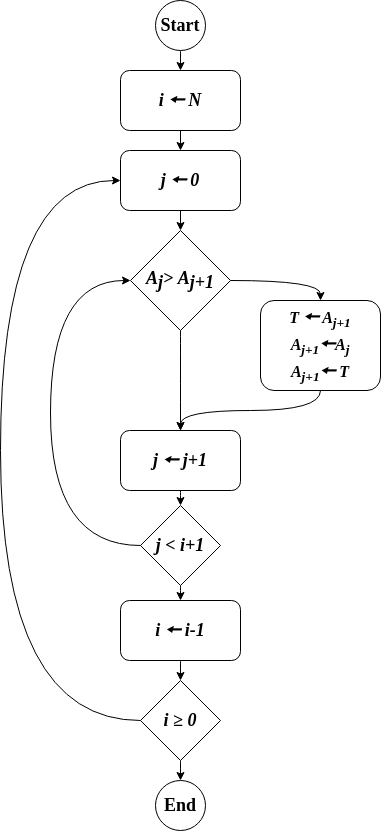
\includegraphics[width=\textwidth]{Chapter2/cfg.png}
      \vspace*{-5mm}
      \caption{Control Flow Graph of bubblesort algorithm [Algorithm \ref{algo:bubble}]}
      \label{fig:cfg}
      \vspace*{5mm}
    \end{subfigure}
    ~
    \hspace*{5mm}
    \begin{subfigure}[b]{0.35\textwidth}
      \centering
      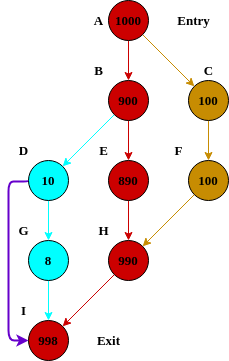
\includegraphics[width=\textwidth]{Chapter2/heatmap-cfg.png}
      \vspace*{-5mm}
      \caption{CFG Heatmap of Algorithm \ref{algo:bubble}. In 1000 runs, different paths are discovered.}
      \label{fig:cfg-heat}
      \vspace*{5mm}
    \end{subfigure}
  \end{adjustbox}
  \caption{Control Flow Graph}
  \label{fig:cfgs}
\end{figure}

% !
% Two types of vulnerabilities: for finding performance problems and the ones causing a crash.
Denial of service (DoS) is a category of vulnerabilities through network that prevents services from correctly responding back to the users. \say{There are many ways to make a service unavailable for legitimate users by manipulating network packets, programming, logical, or resources handling vulnerabilities, among others. If a service receives a very large number of requests, it may cease to be available to legitimate users. In the same way, a service may stop if a programming vulnerability is exploited, or the way the service handles resources it uses} \cite{dos}. In software domain, the vulnerability is either due to an early termination through a crash, or the program terminates with a timeout.

The vulnerabilities arise after target program executes with a triggering input. Miller introduced fuzz testing to examine the vulnerabilities of a collection of Unix utilities \cite{miller1990empirical}. The results showed that a random fuzzing on different versions of the utilities could discover bugs in 28\% of the targets. The automation in testing programs helps the researchers with validating the reliability of a program. The early fuzzers mimic a procedure of searching for the bugs by starting with \textit{identification} of the target program and its inputs. Next, the fuzzing loop initiates, and the program is run with fuzzed inputs as long as the fuzz testing is not terminated. Figure \ref{fig:fuzz_phases} depicts the fuzz testing procedure defined by Sutton et al. \cite{sutton2007fuzzing}. Based on the definitions, a standard fuzzer consists of:

\begin{itemize}
    \item Target identification
    \item Inputs identification
    \item Fuzzed data generation
    \item Execution of target with fuzzed data
    \item Exceptions monitoring
    \item Exploitability determination
\end{itemize}

\begin{figure}[!b]
  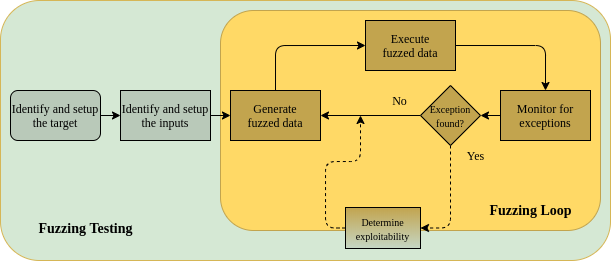
\includegraphics[width=\textwidth]{Chapter2/FuzzingPhases.png}
  \centering
  \caption{Fuzzing phases. Inspired by the definition of Sutton et al. \cite{sutton2007fuzzing}}
  \label{fig:fuzz_phases}
\end{figure}

\textbf{Target} is a software or a combination of executables and hardware \cite{song2019periscope}. A targeted software is any program that a machine can execute. 
Fuzzer needs to know the command for executing the target program and the inputs (arguments) of the program. \textbf{Inputs} are a set of environmental variables, file formats, and any other parameters that affect the execution. The initial seeds of the inputs can guide the fuzzer for finding more complex test cases, yet, it is not mandatory to provide seeds, and a fuzzer can generate valid inputs \textit{out of thin air} \cite{out_of_thin_air}. After the initial setup, the \textbf{fuzzing loop} begins iterating. In each iteration the fuzzer \textbf{executes} the target with the \textbf{provided test cases}. Fuzzer then proceeds to detect exceptions returned from the executions, and considers the executed input responsible for causing a \textbf{vulnerability}. The vulnerability can then be analyzed for \textbf{exploitability} in the last stage. An exploitable vulnerability can compromise the system and initiate an anomaly.

The categories for fuzzers with different \textbf{program awareness} and different \textbf{techniques for fuzzing} the inputs help the community find different applications of the fuzzers for discovering more vulnerabilities. For instance, a developer uses a whitebox fuzzer to assess the immunity of the program (source-code accessible) against malicious activities. On the other hand, an attacker may use a blackbox fuzzer to attack a remote program blindly. A researcher may use a coverage-based fuzzer to consider the execution paths as a variable to reach more regions of the code and detect more crashes; hence, another researcher may use a performance fuzzer to reveal the test cases causing performance issues. 

\subsection{Program awareness}

% It must be explained in more details that these colorful categories are not accurate. 

The \textit{colorful} representation of fuzzers depends on the amount of information collected from a symbolic/concrete execution. A blackbox fuzzer does not gather any information from the execution. In contrast, whitebox fuzzers have all the required access to the program's source code, and greybox fuzzing covers the gray area between the mentioned types.

% Executes a lot - Easily scaled - No program awareness
% Shallow bugs
% Blackbox fuzzer
\subsubsection{Blackbox fuzzing}

Blackbox fuzz testing is a general method of testing an application without struggling with the analysis of the program itself. The target of an analysis executes after calling the proper API's, and the errors are expected to occur in the procedure of trying various inputs. Blackbox fuzzing is an effective technique though its simplicity \cite{woo2013scheduling}.

The introduced fuzzer by Miller \cite{miller1990empirical} was of the very first naive blackbox fuzzers. It runs the fuzzing for different lengths of inputs for each target (of the total 88 Unix utilities) and expects a \textbf{crash}, \textbf{hang}, or a \textbf{succeed} after the execution of the program. Each input is then fuzzed with a random mutation to generate new test cases. One of the \textbf{downsides} of blackbox fuzzing is that the program may face branches with \textit{magic values}, constraining the variables to a specific set of values; for instance, as shown in Listing \ref{lst:magic}, the chance of satisfying the equation $\texttt{magic\_string=="M4G!C"}$ and taking the \texttt{succeed()} path is almost zero. In \cite{banks2006snooze} and \cite{gascon2015pulsar} a set of network protocols are fuzzed in a blackbox manner, but as the target is specified, the performance is enhanced drastically. Any application on the web may be considered a blackboxed program as well, so as \cite{doupe2012enemy} and \cite{duchene2012xss} have targeted web applications and found ways to attack some the websites, looking for different vulnerabilities, such as XSS.

\begin{lstlisting}[language=C++,style=CodeStyle,caption=Magic Value: \texttt{M4G!C} is a magic value,label={lst:magic}]
  string magic_string = random_string();
  if(magic_string == "M4G!C")
      return succeed();
  else
      return failed();
\end{lstlisting}

A blackbox fuzzer is unaware of the program's structure and cannot monitor it's execution. The \textbf{benefit} of using a blackbox fuzzer is the speed of test case generation; the genuine compiled target program is being tested and the fuzzer does not put an effort on processing the inputs and executions. In addition, a blackbox fuzzer is featured to target external programs by using the standard interfaces of those programs. For instance, IoTFuzzer \cite{chen2018iotfuzzer} is an Internet of Things (IOT) blackbox fuzzer, \say{which aims at finding memory corruption vulnerabilities in IoT devices without access to their firmware images.} 
In a recent research by Mansur et al. \cite{mansur2020detecting}, they introduce a blackbox fuzzing method for detecting bugs in Satisfiability Modulo Theories (SMT) problems. As a result, blackbox fuzzing suggests a general solution in diverse domains. On the other hand, one of \textbf{drawbacks} of using blackbox fuzzing is that it finds \textit{shallow} bugs. A shallow vulnerability is an error that appears in the early discovered basic blocks in the CFG of the program. The reason behind this disadvantage is that blackbox fuzzing is \textbf{blind} in understanding the execution, and cannot analyze the CFG.

% Whitebox fuzzers

\subsubsection{Whitebox fuzzing}

Whitebox fuzzing works with the source code of the target. The source code contains the logic of the program and can anticipate the executions' behavior without executing the program (concretely). Symbolic execution \cite{king1976symbolic} is a reliable whitebox fuzzing strategy that analyzes the source code. This analysis replaces the variables with symbols that consider the constraints for each data. This technique helps its fuzzer discover inputs that increase code coverage by discovering new branches after conditional instructions were satisfied. This method detects \textit{hidden} bugs faster due to the powerful constraint solvers \cite{godefroid2008automated}. Although the symbolic execution can solve the conditional branching theoretically, this technique suffers from \textit{path explosion} problem. As an example, in Figure \ref{fig:pathx} a sample section of a program containing a \texttt{loop} and an \texttt{if} statement within the loop. Figure \ref{fig:pathx3} shows the tree of the actions taken until the program reaches the basic block $X$. Solving the current loop requires an exponentially growing number of paths that the fuzzer needs to visit. Whitebox fuzzing is not very practical in the industry as it is expensive (time-consuming / resource-consuming) and requires the source code, which may not be available for testers.

\begin{figure}[!b]
  \begin{adjustbox}{center,max width=1.3\textwidth}
      \begin{subfigure}[t]{0.30\textwidth}
          \centering
          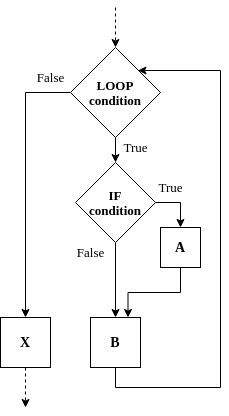
\includegraphics[width=\textwidth]{Chapter2/path-explosion.png}
          \vspace*{-5mm}
          \caption{Path explosion}
          \label{fig:pathx}
          \vspace*{5mm}
      \end{subfigure}
      ~
      \begin{subfigure}[b]{0.80\textwidth}
          \centering
          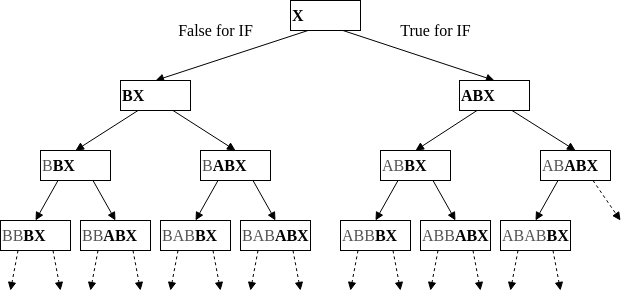
\includegraphics[width=\textwidth]{Chapter2/path-explosion-tree.png}
          \vspace*{-5mm}
          \caption{Path explosion tree}
          \label{fig:pathx3}
          \vspace*{5mm}
      \end{subfigure}
  \end{adjustbox}
  \caption{Path explosion example}
  \label{fig:path}
\end{figure}

SAGE \cite{godefroid2012sage}, a whitebox fuzzer, was developed as an alternative to blackbox fuzzing to cover the lack of blackbox fuzzers \cite{cadar2011symbolic}. It can also use dynamic and \textit{concolic execution} \cite{stephens2016driller} and use taint analysis to locate the regions of seed files influencing values used by the program \cite{ganesh2009taint}. Concolic execution is an effective combination of symbolic execution and concrete (dynamic) executions; in a dynamic execution the fuzzer executes the program and analyzes the run. Godefroid et al. \cite{godefroid2008grammar} have also introduced a whitebox fuzzer that investigates the grammar for parsing the input files without any prior knowledge.

\subsubsection{Greybox fuzzing}

Greybox fuzzing resides between whitebox and blackbox fuzzing, as it has partial knowledge (awareness) about the internals of the target application. The source code is not analyzed, but the executions of the binary files are the main data source for discovering the vulnerabilities in action; the actual application's logic is not considered for the analysis, but the instructions illustrate an overview of the compiled program's logic. A concrete execution of a program represents a reproducible procedure that is executed and can be monitored for its behavior detection. Greybox fuzzer obtains the runtime information from the code instrumentation, and by using other techniques such as taint analysis, concolic executions (obtaining the logic from the binary), and methods for acquiring more information after the \textbf{partial knowledge} of the program \cite{liang2018fuzzing,choi2015dynamic}. 

The code coverage is a viable feature for detecting the new paths that the fuzzer never executed. Registering new paths for testing helps fuzzers in finding different regions of the code for potential vulnerabilities. Later the fuzzer tests the input that caused the new path to check if fuzzing the input can reveal a new vulnerability after constructing tweaked inputs out of the current input. This loop of testing the different inputs continues until specific termination signals show up. AFLGo \cite{bohme2017directed} is a greybox fuzzer that tries digging into the deeper application's basic blocks so that it can reach a specific region. AFLGo focuses on fuzzing more of the inputs that guide the execution as it gets closer to the specified region. This greybox fuzzer shows effective performance in testing a program for detecting errors in new patches of an application and helps with crash reproduction. Another greybox fuzzer, VUzzer \cite{rawat2017vuzzer} enhances the instrumentation to collect control- and data-flow features, which leads to guiding the agnostic fuzzer to find more \textit{intersting} inputs, with less effort (fewer trials of the fuzzed inputs). The core feature in a greybox fuzzer is the \textit{application agnosic} characteristic that targets any executable and observable program in the fuzzer's environment.

\subsection{Input generation}

Greybox fuzz testing requires features to distinguish between various inputs and pick the test cases that help the fuzzer find bugs. Code coverage is a distinguishing feature for preference over the inputs. As described before \ref{sec:2.2.1}, code coverage summarizes the behavior of an execution, and does not analyze the instructions, instead, the graph of the basic blocks (CFG) is analyzed. For \textbf{coverage-guided} fuzzing, the corpus of inputs extends as the fuzzer finds new \textit{execution paths}. On the other hand, a \textbf{performance-guided} fuzzer seeks \textit{resource-exhaustive procedures}.

\subsubsection{Coverage-guided fuzzing}

Coverage-based fuzzing is a technique for fuzz testing that instruments the target without analyzing the logic of the program. In a greybox and whitebox coverage-based fuzzing, the instrumentation detects the different paths of the executions \cite{liang2018fuzzing}. The applied instrumentation collects runtime information such as data coverage, statement coverage, block coverage, decision coverage, and path coverage \cite{yang2009survey}. Bohme et al. \cite{bohme2017coverage} introduced a coverage-based greybox fuzzer that benefits from the Markov Chain model. The fuzzer calculates the \textit{energy} of the inputs based on the \textbf{potency of a path for discovery of new paths}. Later, the inputs with higher energy add more fuzzed inputs to the queue.

Steelix \cite{li2017steelix} is a coverage-guided greybox fuzzer. It implements a coverage-based fuzz testing that is boosted with a \textit{program-state based} instrumentation for collecting the \textit{comparison progress} of the program. The comparison progress keeps the information about \textit{interesting comparisons}. The heavy-weight fuzzing process of Steelix contains an initial light-weight static analysis of the binary. The static analysis returns the basic block and comparison information. Later, the concrete execution of the fuzzed test cases determines the state of the program based on the triggered comparison jumps. In addition to the coverage increasing generation of inputs, Steelix knows how to solve the \textit{magic} comparisons, and looks for new states of the program based on the resolved comparisons.

The code coverage is measured by considering a light-weight instrumentations. This method helps fuzzing to monitor the program without changing the program's resource usage (time, memory, etc.) by a noticeable amount. Hence, due to unaccessibility to the source code, dynamic instrumentation is used as a reliable technique for collecting the runtime information. The trade off for using DI is the increasing performance cost; for instance, QEMU costs 2-5x slower executions \cite{afl_qemu}.

\begin{table}[!t]
  \begin{adjustbox}{width=\linewidth}
    \begin{tabular}{|l|l|l|l|} 
    \hline
Types            & Benefits                                                                                     & Limitations                                                                              & Example Fuzzers                                         \\ 
    \hline
    Whitebox & Deep/Hidden bug finding                                                                      & \begin{tabular}[c]{@{}l@{}}- Path Explosion\\- Accessibility to source code\end{tabular} & \begin{tabular}[c]{@{}l@{}}SAGE\\BuzzFuzz\end{tabular}  \\ 
    \hline
    Blackbox & \begin{tabular}[c]{@{}l@{}}- Fast test case generation\\- General applicability\end{tabular} & \begin{tabular}[c]{@{}l@{}}- Shallow bug finding\\- Blind\end{tabular}                   & \begin{tabular}[c]{@{}l@{}}LigRE\\Storm\end{tabular}    \\ 
    \hline
    Greybox  & \begin{tabular}[c]{@{}l@{}}- Deep bug finding\\- General applicability\end{tabular}          & \begin{tabular}[c]{@{}l@{}}- Access to binary\\- Requires instrumentation\end{tabular}   & \begin{tabular}[c]{@{}l@{}}AFL\\LibFuzzer\end{tabular}  \\
    \hline
    \end{tabular}
  \end{adjustbox}
  \caption{Program awareness for fuzzing}
  \label{table:aware-fuzzers}
\end{table}

\subsubsection{Performance-guided fuzzing}

\begin{table}[!t]
  \begin{adjustbox}{width=\linewidth}
    \begin{tabular}{|l|l|l|l|} 
      \hline
      Types              & Features                                                                                         & Drawbacks                                                             & Examples                                                             \\ 
      \hline
      Coverage-guided    & \begin{tabular}[c]{@{}l@{}}Light-weight\\instrumentation\end{tabular}                            & \begin{tabular}[c]{@{}l@{}}Low guidance\\measurements\end{tabular}    & \begin{tabular}[c]{@{}l@{}}AFL\\LibFuzzer\\Honggfuzz\end{tabular}    \\ 
      \hline
      Performance-guided & \begin{tabular}[c]{@{}l@{}}- More features for guidance\\- Find resource-exhaustion\end{tabular} & \begin{tabular}[c]{@{}l@{}}Heavy weight\\instrumentation\end{tabular} & \begin{tabular}[c]{@{}l@{}}SlowFuzz\\PerfFuzz\\MemLock\end{tabular}  \\
      \hline
    \end{tabular}
  \end{adjustbox}
  \caption{Input generation techniques for fuzzing}
  \label{table:input-gen}
\end{table}  

To enhance the capability of a coverage-based fuzzer, a performance-guided fuzzing technique collects resource-usage information, and leverages code coverage techniques for exploring the CFG. SlowFuzz \cite{petsios2017slowfuzz} is a performance-guided coverage-based greybox fuzzer, which measures the length of the total execution path. SlowFuzz has an interest in evolving the corpus of test cases to discover new paths or generate more resource exhaustive executions. Another performance-guided fuzzer, PerfFuzz \cite{lemieux2018perffuzz} aims to generate inputs for executions with higher \textbf{execution time} by counting the number of times each edge (jump out of basic block) of the CFG is visited. Next, inputs with higher edge counts take more effect on the corpora's evolution. These two performance fuzzers can detect pathological inputs related to CPU usage. Memlock \cite{wen2020memlock} guides the performance of the fuzzing to produce memory-exhaustive inputs. It investigates memory usage by calculating the maximum runtime memory required during executions. MemLock uses static performance instrumentations for profiling memory usage.

% \vspace{1.5\baselineskip}